\section{Aufgabe 5.3}
Wie in den vorherigen Aufgaben und Ausarbeitungen gezeigt, lassen sich mit Hilfe von FEMM sehr gute Simulationen von Plattenkondensatoren erzeugen. Aber auch Kugelkondensatoren lassen sich mit FEMM simulieren und berechnen. \\
Die Methode \texttt{spherecapacity.m}, die im Anhang zu finden ist, nimmt die zwei Parameter $R_1$, der den Innenradius beschreibt und $\varepsilon_r$, das die relative Permittivität des Dielektrikums darstellt, entgegen. Aus der Aufgabenstellung geht hervor, dass für den zweiten zur Berechnung der Kapazität benötigten Parameter $R_2 = R_1 + \SI{7}{\centi\meter}$ gilt. $R_2$ ist der Außenradius des Kugelkondensators. Optional könnte man die Methode auch so schreiben, dass $R_2$ übergeben werden kann.\\
Im Vergleich zu den bisherigen Simulationen in FEMM haben wir nun kein planares Problem mehr, sondern ein achsensymmetrisches. In der Problemdefinition (Zeile 6) wird deshalb ein \texttt{'axi'} übergeben. Damit wird bestimmt, dass sich die erzeugte Fläche in Abbildung \ref{fig:KK} nicht in die Tiefe entwickelt, sondern um die z-Achse gedreht wird. Dadurch erhält man eine 3-Dimensionale Kugel, die FEMM zwar nicht darstellen, aber berechnen kann.\\ \\
Zunächst werden zwei Halbkreise erzeugt (Zeile 12-26), zwischen diesen beiden Halbkreisen liegt eine Spannungsdifferenz von \SI{1}{\volt} an. Des Weiteren werden zwei Blocklabel erstellt (Zeile 28 und 31), das erste Label liegt zwischen den beiden Halbkreisen und beinhalten die Informationen über die relative Permittivität des Dielektrikums. Mit dem zweiten Label wird sichergestellt, dass nur die von den beiden Halbkreisen und deren Verbindungslinien eingeschlossene Fläche bei der Berechnung berücksichtigt wird. Hierzu wird dem Label die Property \texttt{'<No Mesh>'} übergeben. Schließlich werden die Verbindungslinien zwischen den Halbkreisen erstellt(Zeile 38 und 39), um eine abgeschlossene Fläche zu erzeugen. \\ \\
\begin{figure}[h]
	\centering
	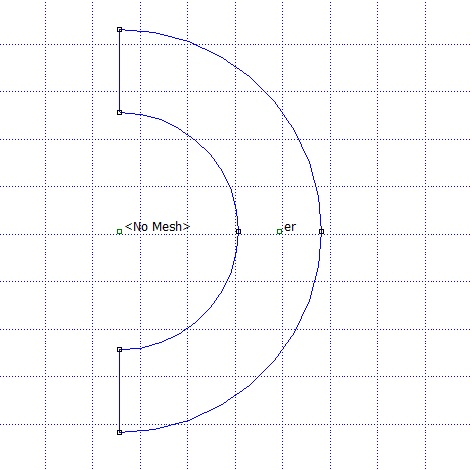
\includegraphics[width=.45\textwidth]{data/Kugelkondensator}
	\caption{Ein mit Hilfe der Routine \texttt{spherecapacity.m} erzeugter Kugelkondensator mit $R_1 = \SI{7}{\centi\meter}$ }
	\label{fig:KK}
\end{figure}

Mit 
\begin{equation}
	C = 4\pi\varepsilon_0\varepsilon_r\frac{R_2R_1}{R_2-R_1}
	\label{eq:Kapa}	
\end{equation}
lässt sich die Kapazität eines homogenen Kugelkondensators berechnen.
Um den Einfluss der Radien auf die Kapazität zu untersuchen, wurden der Methode \texttt{spherecapacity.m} 100 verschiedene Radien $R_1 \in \mathbb{N}, R_1 \in [1,100]$, mit der Einheit \si{\centi\meter} übergeben. Für den Radius $R_2$ gilt weiterhin
\begin{equation}
	R_2 = R_1 + \SI{7}{\centi\meter}.
	\label{eq:R2}
\end{equation}
Die berechneten Kapazitätswerte sind in Abbildung \ref{fig:Kapa} graphisch dargestellt. Die Formel 
\begin{equation}
	C = 4\pi\varepsilon_0\varepsilon_r\frac{(R_1+\SI{7}{\centi\meter})R_1}{R_1+\SI{7}{\centi\meter-R_1}}
\end{equation}
ergibt sich indem man (\ref{eq:R2}) in (\ref{eq:Kapa}) einsetzt. Durch weiteres vereinfachen folgt, dass die Kapazität
\begin{equation}
	C = 4\pi\varepsilon_0\varepsilon_r\frac{R_1^2+\SI{7}{\centi\meter}}{\SI{7}{\centi\meter}}
\end{equation}
quadratisch von $R_1$ abhängt, dies erklärt den quadratischen Verlauf der Kapazität (Abbildung \ref{fig:KK}) des Kugelkondensators mit steigendem Innenradius.

\begin{figure}
	\centering
	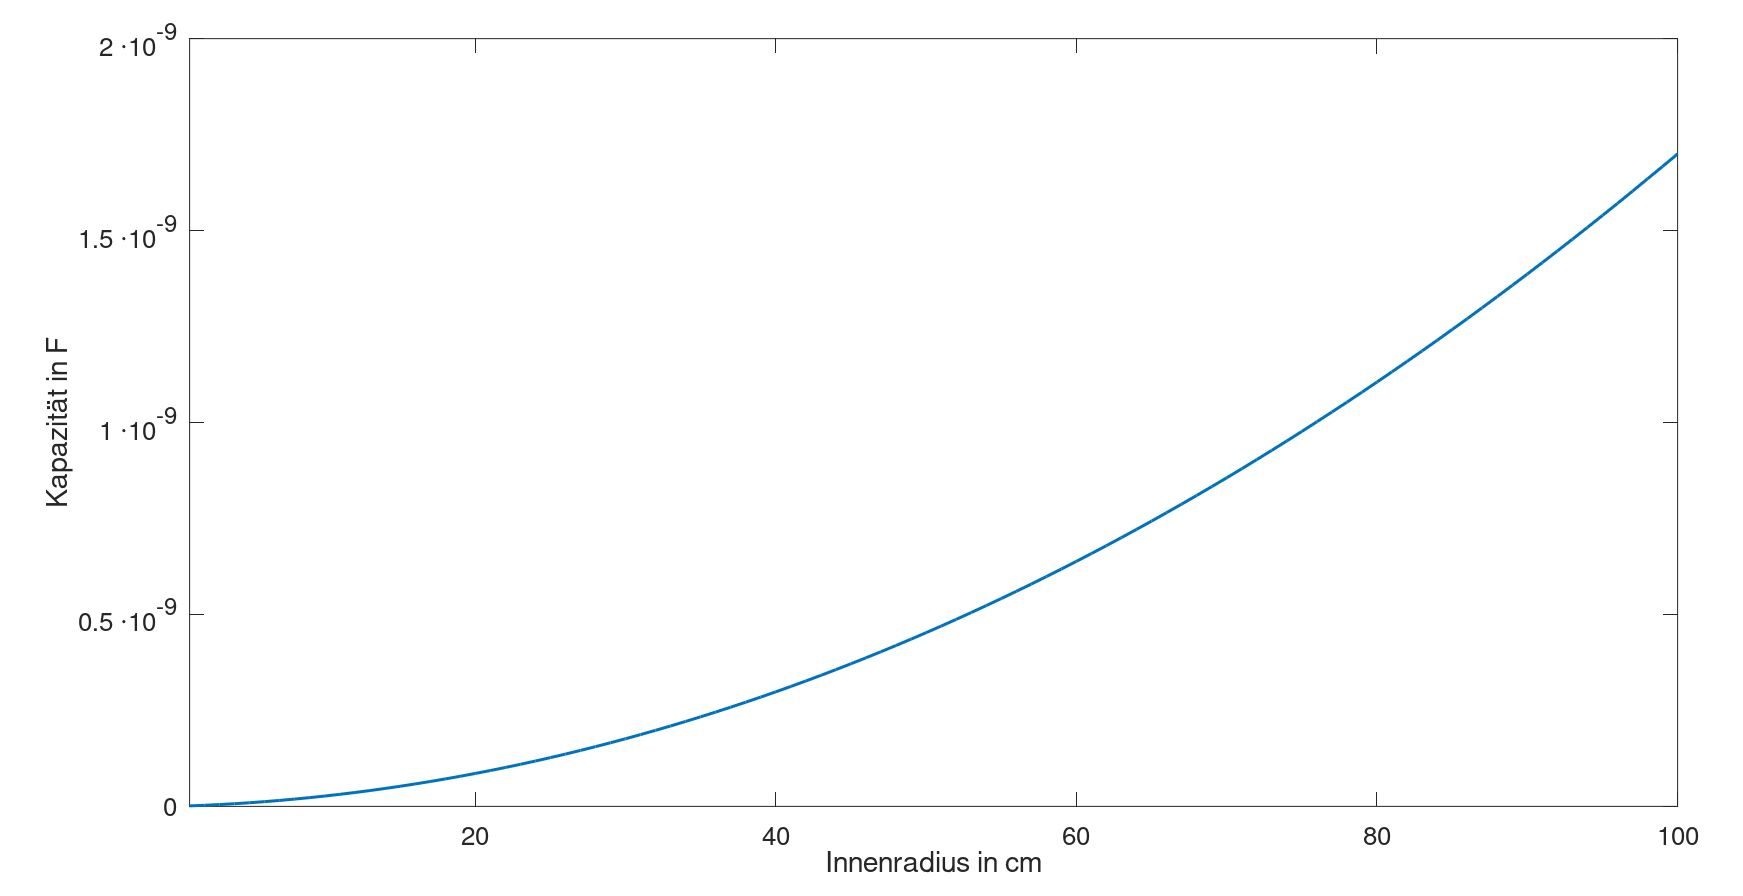
\includegraphics[width=\textwidth]{data/Kugelkapa}
	\caption{Verlauf der Kapazität mit steigendem Radius $R_1$ und $R_2 = R_1 + \SI{7}{\centi\meter}$}
	\label{fig:Kapa}
\end{figure}
\newpage
Unter der Voraussetzung, dass $(R_2+R_1) = \SI{15}{\centi\meter}$ gilt, beträgt der Innenradius $R_1 = \SI{4}{\centi\meter}$ und der Außenradius $R_2 = \SI{11}{\centi\meter}$. Analytisch lässt sich mit (\ref{eq:Kapa}) eine Kapazität $C_{\mathrm{ana}} = \SI{6,994}{\pico\farad}$ berechnen, FEMM berechnet eine Kapazität $C_{\mathrm{num}} = \SI{6,986}{\pico\farad}$. \\ \\
Der relative Fehler
\begin{equation}
	\mathrm{err :=} \frac{|C_{\mathrm{ana}}-C_{\mathrm{num}}|}{|C_{\mathrm{ana}}|}
	\label{eq:err}
\end{equation}
ergibt sich mit den vorher berechneten Werten $C_{\mathrm{ana}}$ und $C_{\mathrm{num}}$ zu $1.1 \cdot 10^{-3}$, liegt also im niedrigen Promillebereich. Die durch FEMM berechnete Annäherung ist sehr exakt.